\documentclass[tikz,border=2pt]{standalone}
\usepackage{amsmath}
\usetikzlibrary{arrows.meta,decorations.pathreplacing}
\begin{document}
% Kendall's notation A^B/Y^C/c/K mapped onto one station: arrivals (inter-arrival law A, batch
% size B), a FIFO queue, c parallel servers (service law Y, service batch C), system size K.
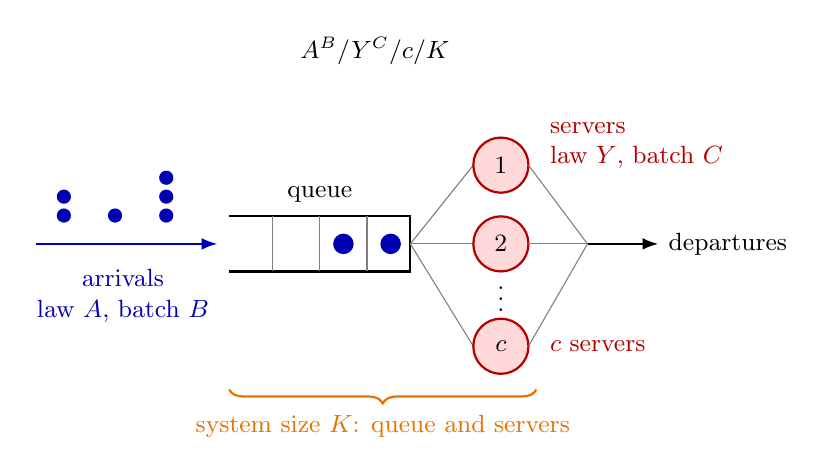
\begin{tikzpicture}[font=\small, >={Latex[length=2mm]}]
  \node at (4.3,2.45) {$A^{B}/Y^{C}/c/K$};
  % arrivals in batches
  \draw[->, blue!70!black, thick] (0,0) -- (2.3,0);
  \foreach \x/\n in {0.35/2, 1.0/1, 1.65/3}
    \foreach \i in {1,...,\n}
      \fill[blue!70!black] (\x,{0.12+0.24*\i}) circle (0.09);
  \node[blue!70!black, anchor=north, align=center] at (1.1,-0.2) {arrivals\\law $A$, batch $B$};
  % queue
  \draw[thick] (2.45,0.35) -- (4.75,0.35) -- (4.75,-0.35) -- (2.45,-0.35);
  \foreach \x in {3.0,3.6,4.2} \draw[gray] (\x,0.35) -- (\x,-0.35);
  \foreach \x in {3.9,4.5} \fill[blue!70!black] (\x,0) circle (0.13);
  \node[anchor=south] at (3.6,0.4) {queue};
  % servers
  \foreach \y/\lab in {1.0/1, 0/2, -1.3/c} {
    \draw[gray] (4.75,0) -- (5.55,\y);
    \draw[red!70!black, thick, fill=red!15] (5.9,\y) circle (0.35);
    \node at (5.9,\y) {$\lab$};
    \draw[gray] (6.25,\y) -- (7.0,0);
  }
  \node at (5.9,-0.6) {$\vdots$};
  \node[red!70!black, anchor=west, align=left] at (6.4,1.25) {servers\\law $Y$, batch $C$};
  \draw[->, thick] (7.0,0) -- (7.9,0) node[anchor=west] {departures};
  % system size
  \draw[orange!90!black, thick, decorate, decoration={brace, amplitude=5pt, mirror}]
    (2.45,-1.85) -- (6.35,-1.85);
  \node[orange!90!black, anchor=north] at (4.4,-2.05) {system size $K$: queue and servers};
  \node[red!70!black, anchor=west] at (6.4,-1.3) {$c$ servers};
\end{tikzpicture}
\end{document}
